\subsubsection{OLS, Ridge and lasso: the relation between betas, lambdas and complexity}
We begin by examining the performance of the regression model on synthetic, uniformly distributed data. Figure \ref{fig:ols mse} shows that for OLS, the MSE decreases as the polynomial degree of the design matrix increases. The reduction is most significant from degree 0 to 1, with a drop of approximately 0.9, compared to a smaller reduction of about 0.3 between degrees 1 and 5. A similar trend is observed in the R² scores, shown on the right side of Figure \ref{fig:ols mse}, where the score increases by 0.6 from degree 0 to 1, and by 0.2 between degrees 1 and 5. The sharp improvement from degree 0 to 1 is expected as the Franke Function takes two input variables, making it difficult to model using only one. The gradual improvement from degrees 1 to 5 is also expected, as the addition of more terms and fine-tuning of the beta values improves model accuracy. However, beyond degree 5, we observe that the OLS model becomes overfitted, indicating that higher polynomial degrees do not improve performance on this data set.

\begin{figure}[H]
     \includegraphics[width=15cm]{Images/OLS_error_degree.png}
     \caption{Performance of OLS as a function of polynomial degrees when uniform data are used.}
     \label{fig:ols mse}
\end{figure}

The corresponding beta values for Figure \ref{fig:ols mse} are shown for different polynomial degrees in Figure \ref{eq:betaOLS}. We observe that both the number of beta values and their variation increase with higher polynomial degrees. More beta values allow the model to capture greater variability in the data, which explains the improved performance with higher degrees. However, by including more polynomial terms, we also introduce collinearity between them as the terms in polynomial regression are powers of each other. This impacts the regression coefficients, so that they become more unstable and sensitive to small changes in the data. \cite{polyreg_budescu} As a result, the beta values can assume large values, which we clearly see on degree 7.  Degree 1 shows the largest performance jump, and the three beta values (in orange) have a small range compared to higher polynomial degrees. For degree 7, when our model is overfitted, the model is so sensitive too small changes in our data that it doesn´t catch the general trend. It no longer benefits from including more beta terms, and the beta values seems to assume arbitrarily large values. 
Although scaling the data can reduce the risk of multicollinearity between our terms\cite{polyreg_budescu}, we saw no effect on our beta plot when we dropped the scaling. This could be due to the fact that our uniform data already have mean zero, so the effect of scaling the design matrix is not visible. 
\begin{figure}[H]
     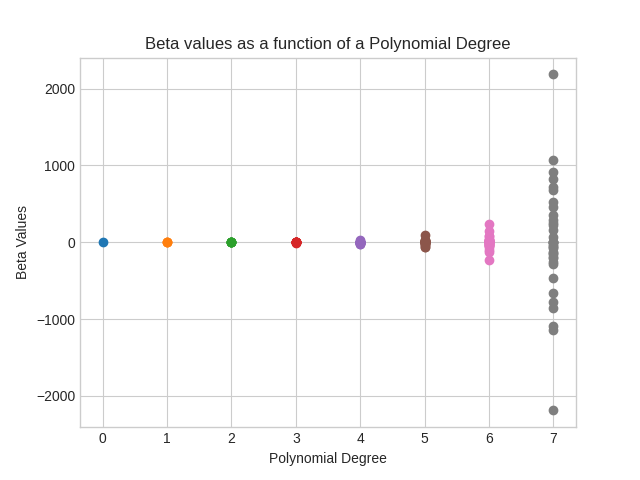
\includegraphics[width=15cm]{Images/beta_ols.png}
     \caption{Betavalues for OLS with uniform data. We can see that the beta values diverge when the polynomial degree increase. Each color represents betavalues for one degree.}
     \label{fig:betavalues_ols}
\end{figure}

Moving on to the results for the Ridge regression, we observe the MSE and $R^{2}$ scores (Figure \ref{fig:ridge mse}). The seven different lambdas are all equal from degree 0 to degree 1, but diverges after that for both MSE and R2. It is clear that the lower the lambda values, the better the Ridge regression model fits this data. Lower lambdas than 1e-05 did not improve the model further, while adding more degrees after nine only improved the performance by negligible amounts. 

\begin{figure}[H]
     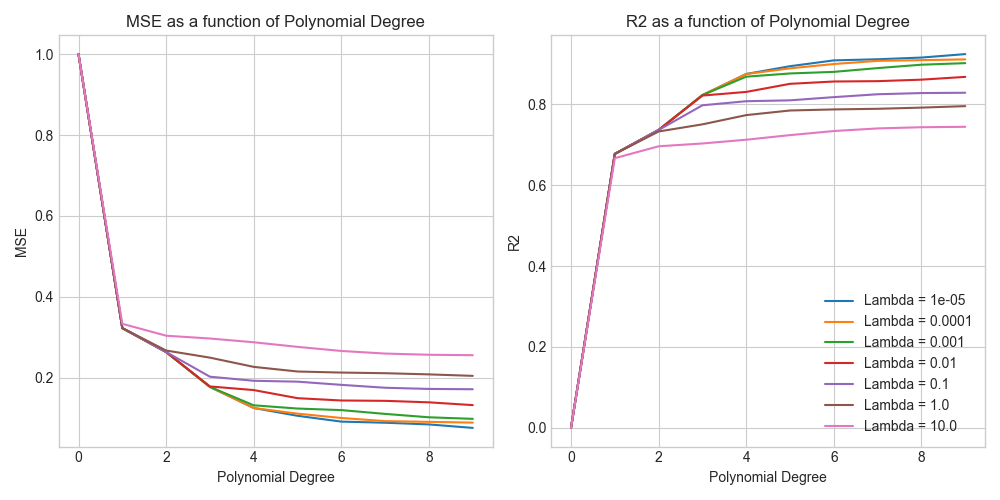
\includegraphics[width=15cm]{Images/ridge_error_degree.png}
     \caption{Performance of Ridge as a function of polynomial degree for different lambdas. On uniform data we see that lambda 1e-05 gives the best performance.}
     \label{fig:ridge mse}
\end{figure}

The results from Lasso regression in Figure \ref{fig:lasso mse} show more variability compared to Ridge. The lambda value of 1e-06 performs best up to degree 5, except for degree 4, and again at degree 8 before overfitting occurs. Lambda 1e-05 performs best for most other degrees, with the exception of degree 4, where 1e-04 is optimal. Overall, 1e-05 appears to be the most stable. We observe that at lower complexities, smaller lambda values perform best. However, as complexity increases, slightly larger lambda values yield the lowest MSE, while the smallest lambdas drop in performance. This happens because larger lambdas strike a better balance between capturing data nuances and avoiding overfitting. \cite{openai2023chatgpt}

\begin{figure}[H]
     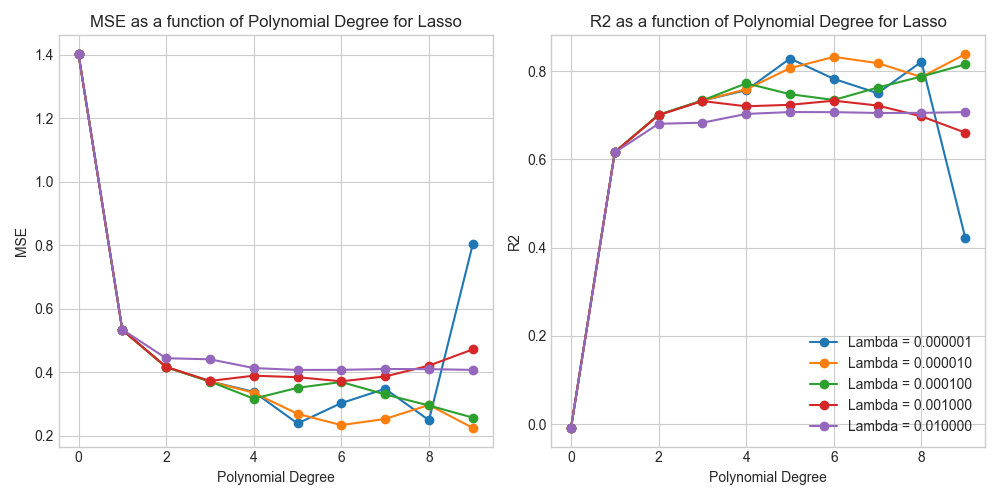
\includegraphics[width=15cm]{Images/lasso_error_degree.png}
     \caption{Performance of Lasso as a function of polynomial degree for different lambdas. On uniform data we see that lambda 1e-05 is performing best.}
     \label{fig:lasso mse}
\end{figure}

When comparing the three regression methods it seems that Ridge is performing best overall, with the lowest MSE and the highest R2 values. It is also the most stable method as the performance increases in proportion to the complexity. We believe Ridge is better than Lasso because the spesific dataset we used is too simple and too small for the more complex Lasso penalty to show it's potential. However, the OLS model overfits the data, so a penalty is beneficial. 

\subsubsection{Bootstrap: bias variance tradeoff}

As we don't have the computational power to show the bias-variance tradeoff for the real data, we present the bootstrap analysis for the synthetic data. We can see from Figure \ref{fig:bootstrap1000samples} that the bias is decreasing as a function of model complexity. In contrast, the variance is increasing with model complexity. As the error can be decomposed to bias and variance, we want to find the optimal balance between the bias and the variance. From our error plots we expected the optimal bias variance tradeoff to be somewhere after degree 8. We observe that it is between degree 10 and 11. For the optimal bias variance trade off, we would choose degree 11. 

\begin{figure}[H]
     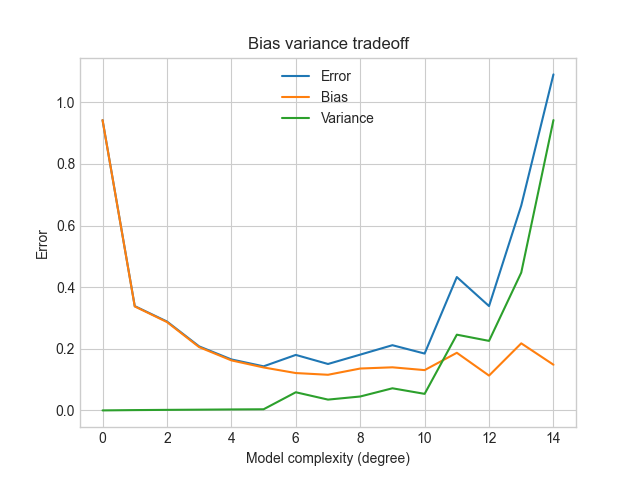
\includegraphics[width=15cm]{Images/uniform_1000_bootstrap.png}
     \caption{Bootstrap of uniform data with 1000 samples (we had to increase the number of samples to see the trade-off) and 100 bootstraps. We can clearly see the bias variance tradeoff at the crossing point between degree 10 and 11.}
     \label{fig:bootstrap1000samples}
\end{figure}

\subsubsection{Comparison of OLS, Lasso and Ridge on terrain data}

One main finding is that our Lasso model, which produced decent recults with a small sample from the uniform distribution, requires a significant amount of computational resources with the high dimensional terrain data. We adjusted the hyperparameters that could affect runtime and tested both locally and on a remote machine, but were not successfull in producing sensible results. However, we can see in Figure \ref{CV_terraindata} that Ridge and Lasso have the most stable performance  with increasing polynomial degree. OLS on the other hand have a rapidly increasing MSE after degree 5. 

\begin{figure}[H]
     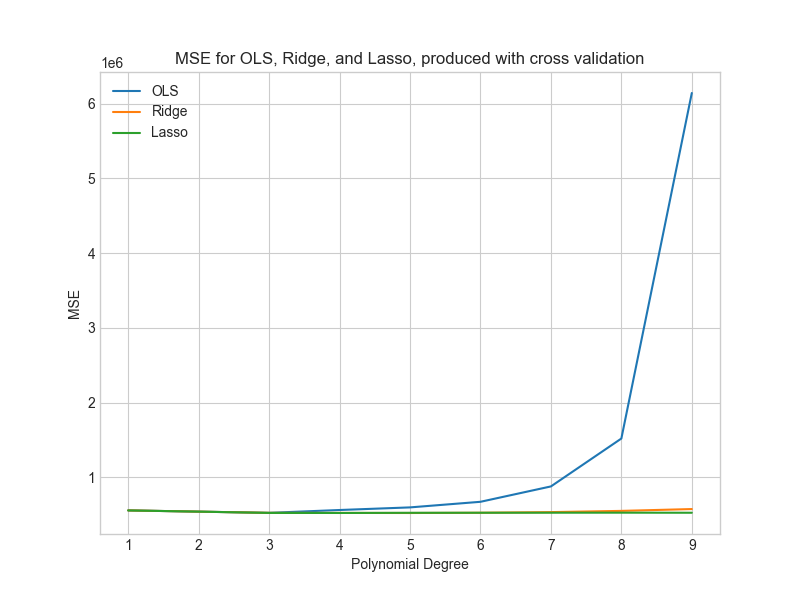
\includegraphics[width=\textwidth]{Images/CV_terrain_data.png}
     \caption{MSE after cross validation showing that OLS is least stable in increasing model complexity. The plot is based on terrain data.}
     \label{CV_terraindata}
\end{figure}

Because Lasso was the best performing model on the terrain data in terms of producing stable results with increasing complexity, we decided to compare the heatmap of the terrain data in Figure \ref{terrain data heatmap comparison} and the reproduction from Lasso in Figure \ref{fig:Lasso CVHeatmap} using cross validation. We were hoping to be able to recreate some of the terrain data, but we can see that the reproduction doesn´t capture the terrain data, only the gradient shadow. This is supported by the relatively high MSE. It should again be noted that because of the lack of computational resources we are not able to explore the increase of model complexity, which is a weakness with the comparison. In Appendix A we have included heatmaps in Figure \ref{fig:four graphs} for the three regression methods computed without cross validation to show that it is possible to get better reproductions on this data, but not without overfitting it. 

\begin{figure}[H]
     \begin{subfigure}[h]{0.45\textwidth}
         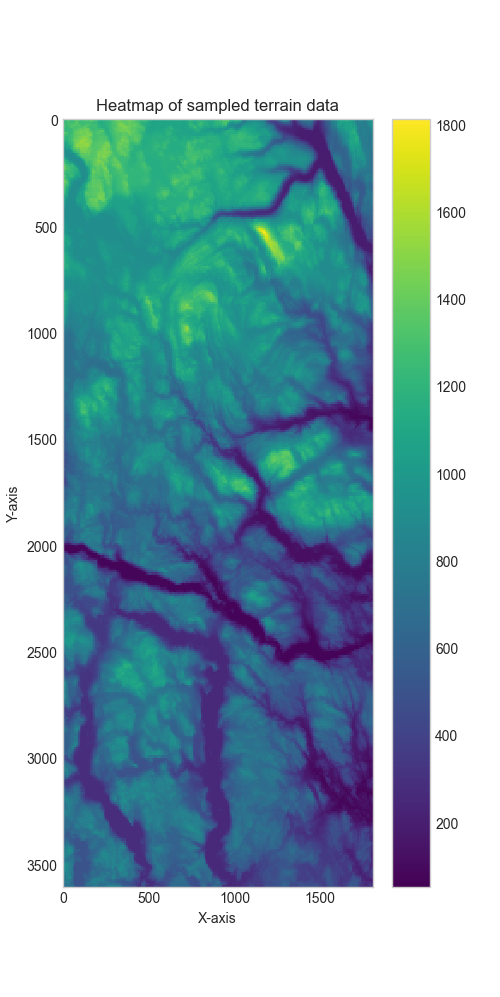
\includegraphics[width=\textwidth]{Images/sampled_data_heatmap.png}
         \caption{Original sampled data}
         \label{terrain data heatmap comparison}
     \end{subfigure}
     \hfill
     \begin{subfigure}[h]{0.45\textwidth}
         \centering
         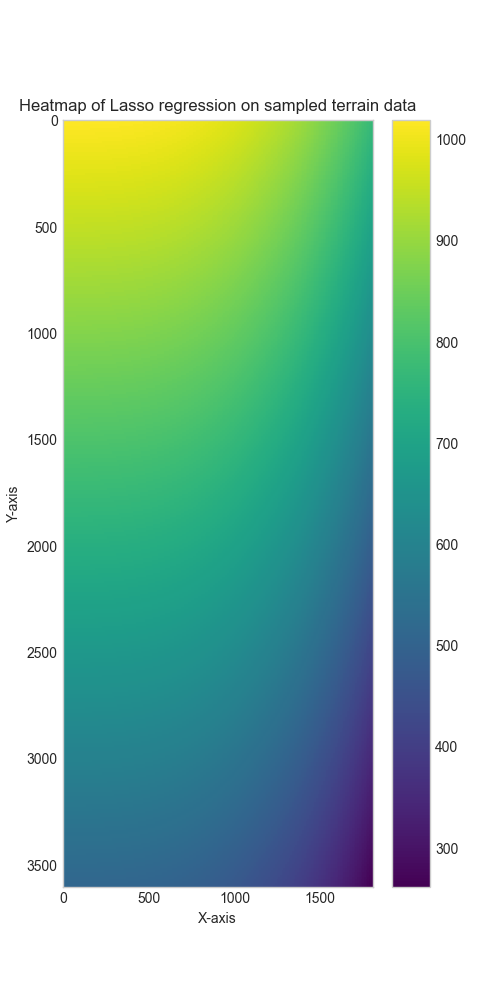
\includegraphics[width=\textwidth]{Images/cv_lasso_terrain_heatmap.png}
         \caption{Lasso}
         \label{fig:Lasso CVHeatmap}
     \end{subfigure}
     
        \caption{Heatmaps showing the true terrain side by side with the terrain estimated by the Lasso model. The Lasso model is chosen through cross validation. We see that by emphasizing that it should generalize to new data, it is not able to recreate our original terrain data.}
        \label{fig:four graphs}
\end{figure}

